\chapter{Accounts}\label{chapter.accounts}

It is time to take a step back and look at the construction we've built. A chain
is used to order transactions into a ledger $L$. From this ledger of transactions we can deduce
a state, which is a UTXO set. This state is obtained as follows. We start with the initial
state $\st_0 = \{\,\}$, the empty UTXO map. We then apply each transaction in the ledger
one-by-one as illustrated in \Cref{fig.state-transition}.
To apply a transaction $\tx_i$, we take the previous state $\st_{i-1}$ and modify
it, according to what the transaction does, to obtain the next state $\st_i$. The way the
transaction acts on the state is by consuming some UTXOs (which are removed from the state)
and by producing some new UTXOs (which are added to the state). When all transactions have been
applied, we arrive at the final state $\st_{|L|}$.

\begin{figure}[h]
  \centering
  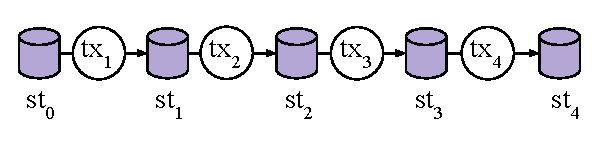
\includegraphics[width=0.7 \columnwidth,keepaspectratio]{09-accounts/figures/tx-state-transition.pdf}
  \caption{Transitioning state by applying transactions.}
  \label{fig.state-transition}
\end{figure}

There are two layers at play here. First, the chain protocol producing blocks and
picking the longest chain. Second, the layer handling the transactions on top. The chain protocol is responsible
for ordering transactions, but is agnostic to the transaction semantics. The transaction semantics
are also agnostic to the chain protocol, relying on it only for ordering. The two layers interoperate
with each other when the chain protocol needs to validate a block, which requires asking the
transaction layer to validate the transactions in the block.
Similarly, when maintaining the mempool, the node checks incoming transaction validity against the mempool state
by attempting to apply the transaction to the current mempool state.
We call the layer responsible for \emph{ordering} transactions the \emph{consensus layer}\index{Consensus Layer},
and the layer responsible for the transaction semantics the \emph{execution layer}\index{Execution Layer}.

\section{The UTXO Transition Function}

In our transaction semantics, we chose to use UTXOs and to have each state represent a UTXO set,
because it was useful for representing ownership. We now observe that these semantics could be
different. We just need to specify what state we start with, and how to transition from state to state.
We call the state we start with the \emph{initial state} $\st_0$, and the way to transition from state
to state the \emph{transition function} $\delta$. The $\delta$ transition function takes a state and
a transaction and returns a new state if the transaction is valid, or $\bot$ otherwise:

\[
  \delta(\st, \tx) = \begin{cases}
    \st' & \text{if $\tx$ is valid w.r.t. $\st$} \\
    \bot & \text{otherwise} \\
  \end{cases}
\]

In the UTXO model which we have already explored in the previous chapters, we can now
write out the $\delta$ function explicitly, as illustrated in \Cref{alg.utxo}.
We call this transition function $\delta_{\textsf{UTXO}}$. This makes precise the informal
validation procedure described in \Cref{sec.transaction.validation}.

\import{./09-accounts/}{algorithms/alg.utxo}

Our function takes as input a state $\st$ and a transaction $\tx$. The state
$\st$ represents the UTXO set with a mapping from \emph{outpoints} to
\emph{outputs}. An outpoint is a tuple $(\txid, \idx)$ where $\txid$ is the
transaction ID and $\idx$ is the index of a transaction output. An output is a
tuple $(\pk, \amount)$ where $\pk$ is the public key of the recipient and
$\amount$ is the amount of money sent. A transaction is a dictionary with
\emph{inputs} and \emph{outputs} fields. The \emph{inputs} field is a list of
outpoints that the transaction consumes. The \emph{outputs} field is a list of
outputs that the transaction produces. We assume that the transaction input to
$\delta$ is well-typed, e.g., that each $\amount$ is non-negative. Of course,
this syntactic validity has to be verified by the implementation.

If you're implementing this, you may be tempted to check all inputs against the
previous UTXO set $\st$ and, after the transaction has been validated, remove
them to produce $\st'$.  A pitfall in this implementation is that it allows two
separate inputs to refer to the same UTXO, a double spending within a single
transaction. It is avoided here by dynamically updating $\st'$ after each input
is checked.

\section{The Accounts Model}

The UTXO model is reminiscent of physical banknotes and coins. Like UTXOs, each banknote or
coin is always spent in its entirety, even though other coins may be given as
change. I can keep track of the balance of my wallet by adding up the values of
all the unspent coins in my wallet. I pay you by transferring the ownership of a
coin to you.

In everyday life, aside from banknotes and coins, we also use bank accounts.
The state of my bank account is described by my balance. The global state of all
bank accounts is a list of an account identifier together with its balance. Each banking
transaction debits one account and credits another account with the same amount
(minus some fees).

Bringing this model to the blockchain world is as simple as defining a different
$\delta$ function. We call this function $\delta_\textsf{accounts}$ which
we will now develop. Similar to the UTXO model, we still
use public/private key pairs to authenticate transactions. It is therefore natural
that an account is identified with a public key. The state is a mapping from public
keys (account identifiers) to a dictionary containing information about the account,
such as its balance, which is simply a non-negative integer. An example accounts model
state is shown in \Cref{tbl.balanceState} (in reality, instead of names, the state keeps
public keys).

\begin{table}[htbp!]
    \centering
    \begin{tabular}{|l|r|}
    \hline
    \textbf{Account} & \multicolumn{1}{l|}{\textbf{Balance}} \\ \hhline{|=|=|}
    Dionysis         & 1                                     \\ \hline
    Odysseas         & 100                                   \\ \hline
    David            & 5                                     \\ \hline
    \end{tabular}
    \caption{Example accounts model state.}
    \label{tbl.balanceState}
\end{table}

A transaction in the accounts
model contains the account being debited (the source), called the \emph{from} field, and the account
being credited (the destination), called the \emph{to} field. It also contains the amount of money being transferred,
the \emph{value} field. Contrary to the UTXO model, the fees cannot be implicitly calculated, and
so must be explicitly included in the transaction as a separate \emph{fee} field, also a non-negative
integer. Finally, the transaction is signed by the source account, and this signature is included in
the transaction as the \emph{signature} field. Of course, similar to the UTXO model, the signature is
made on the \emph{unsigned transaction}, which is the transaction with the signature field set to $\bot$.
An example transaction in the accounts model is shown in \Cref{tbl.accountsTx}.

\begin{table}[htbp!]
\centering
    \begin{tabular}{|l|l|r|r|l|}
         \hline
         \textbf{From} & \textbf{To} & \textbf{Value} & \textbf{Fee} & \textbf{$\sigma$} \\
         \hhline{|=|=|=|=|=|}
         Dionysis & Odysseas & 1 & 0 & $\bot$ \\
         \hline
    \end{tabular}
    \caption{Example unsigned transaction in the accounts model.}
    \label{tbl.accountsTx}
\end{table}

It is simpler to apply a transaction $\tx$ to a state $\st$ in the accounts model than in the UTXO model.
First, we verify the validity of the transaction. Namely, we check that the \emph{from} account has sufficient balance.
Next, we check that the signature validates with the \emph{from} account, which is a public key. Lastly, we
update the balances of both accounts to reflect the transfer.

Unfortunately, we are not done yet.
A problem arises if our accounts transaction is formatted as described above. Imagine that Alice buys coffee
from Eve every morning and that the coffee always costs $5$ units. How would these transactions look like?
They would all be the same! Our ledger must record each of these identical but separate payments individually.

Eve can mount an attack: Simply copy Alice's transaction the next
morning, even though she happened not to buy a coffee, thereby stealing money from Alice. This is a \emph{replay attack}\index{Replay Attack}.

Our system must have a way to distinguish different transactions that share the same \emph{from}, \emph{to},
\emph{value}, and \emph{fee} fields, while protecting against replay attacks. To do this, we simply add a \emph{nonce}
field to the transaction which is an integer associated with the \emph{from} account that starts at $0$ and is incremented
for each new transaction. In the state, we keep track of the current nonce for each account. With this addition, the
final state and transaction structures are depicted in
\Cref{tbl.accountsStateWithNonce,tbl.accountsTxWithNonce}.

\begin{table}[htbp!]
    \centering
    \begin{tabular}{|l|r|r|}
    \hline
    \textbf{Account} & \multicolumn{1}{l|}{\textbf{Balance}} & \multicolumn{1}{l|}{\textbf{Nonce}} \\ \hhline{|=|=|=|}
    Dionysis         & 1                                     & 7 \\ \hline
    Odysseas         & 100                                   & 12 \\ \hline
    David            & 5                                     & 3 \\ \hline
    \end{tabular}
    \caption{Example accounts state with nonces.}
    \label{tbl.accountsStateWithNonce}
\end{table}

\begin{table}[htbp!]
    \centering
    \begin{tabular}{|l|l|r|r|r|l|}
            \hline
            \textbf{From} & \textbf{To} & \textbf{Value} & \textbf{Fee} & \textbf{Nonce} & \textbf{$\sigma$} \\
            \hhline{|=|=|=|=|=|=|}
            Dionysis & Odysseas & 1 & 0 & 8 & $\bot$ \\
            \hline
    \end{tabular}
    \caption{Example accounts transaction with nonces.}
    \label{tbl.accountsTxWithNonce}
\end{table}

Using these nonces, we can now solve the replay problem:
Our system will consider a transaction valid if its nonce is exactly
the next nonce of the \emph{from} account. When the transaction is applied,
the nonce of the \emph{from} account is increment, and thus will never be
considered valid again.

The final transition function $\delta_\textsf{accounts}$ is shown in \Cref{alg.accounts}.

\import{./09-accounts/}{algorithms/alg.accounts}

An example practical system that uses the UTXO model is Bitcoin, whereas Ethereum uses the
accounts model.

We summarize the difference between the two models in \Cref{tbl.UTXOvsAccounts}.

\begin{table}[htbp!]
    \centering
    \makebox[\textwidth][c]{
    \begin{tabular}{|m{3cm}|m{4cm}|m{6.5cm}|}
        \hline
        & \textbf{UTXO} & \textbf{Accounts} \\ \hhline{|=|=|=|}
        \textbf{Real System} & Bitcoin & Ethereum \\
        \hline
        \textbf{Transaction $tx$} & 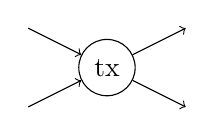
\begin{tikzpicture}[
        txnode/.style={thin,draw=black,circle},
        ]
        \node[txnode] (tx) at (0,0) {tx};
        \draw[->] (-1,0.5) -- (tx);
        \draw[->] (-1,-0.5) -- (tx);
        \draw[->] (tx) -- (1, 0.5);
        \draw[->] (tx) -- (1,-0.5);
        \end{tikzpicture}
        &
        \begin{tabular}{|c|c|c|c|c|c|}
        \hline
        From & To & Value & Fee & Nonce & {$\sigma$} \\
        \hline
        \end{tabular} \\
        \hline
        \textbf{State update} & {Remove consumed outputs and add produced outputs} & {Decrease balance of sender, increase balance of receiver} \\
        \hline
        \textbf{Transaction validation} & {Signature, Inputs exist in $\st$.} & {Signature, Nonce unique.} \\
        \hline
        \textbf{Conservation Law} & {
            $\sum \textsf{in.v} \geq \sum \textsf{out.v}$
        } & {
            $\tx.\textsf{from}.\textsf{balance} \geq \tx.\textsf{value}$
        } \\
        \hline
        \textbf{Fees} & {$\sum \textsf{in.v} - \sum \textsf{out.v}$} & {Explicit $\tx\textsf{.fee}$} \\
        \hline
        \textbf{Initial state} & $\emptyset$ & $\{\}$ \\
        \hline
    \end{tabular}
    }
    \caption{Side by side comparison of the UTXO and accounts models.}
    \label{tbl.UTXOvsAccounts}
\end{table}

Beyond the syntactic differences highlighted in the table, there is a deeper difference between the two models.
In the case of UTXO, when given an unordered set of mempool transactions for which it is guaranteed that there
exists a valid ordering, it is easy to find a valid ordering. Simply topologically sort the transaction graph.
In the case of accounts, one may be tempted to order transactions in a greedy way, namely by including the first
transaction that can validly be included first, followed by the second, and so on. However, this algorithm does
not necessarily always produce a valid ordering of transactions, even if one exists.
It is not obvious how to efficiently find such an ordering.

% TODO(Odysseas): example of orderable accounts transaction set that is not orderable by the greedy algorithm

\section{State Machine Replication}

In our two examples of state transition functions, we have dealt with states encoding money ownership,
albeit in two different formulations. As you may have already imagined, the state collectively maintained
by the nodes can really be any data structure, and not just about money. The transition function
can be any arbitrary computation that allows the state to evolve. The input to that computation,
namely the instructions of \emph{how} the state is supposed to evolve, is the transaction.

What we have really built is a \emph{computer in the sky}\index{Computer in the Sky},
a machinery allowing a mutually distrustful
set of parties to collectively maintain an evolving state. Any party among them can provide an input
to that magical computer, in the form of a transaction, as long as it satisfies a set of mutually preagreed
rules of validity. The computer in the sky will process that input using the state transition function
and evolve its state, making the new state available to all parties observing.

All of these observers will arrive at \emph{consistent} conclusions about the state of the machine,
which is guaranteed by the safety of our consensus layer. Consistency here means that the current state
of the machine observed by all honest parties is not necessarily the same, but that it is not conflicting.
In particular, one party may be ``ahead'' of the other. The party who is ahead has applied more transactions
than the party who is behind. The state of the party who is ahead can be reached by applying those transactions
using the transition function, exactly because the ledger of the party behind is a prefix of the ledger of
the party ahead. These parties hope to agree on the order of transactions in order to arrive at consistent states.
Of course, if we are hoping to reach such consistency, the transition function must be deterministic so that
it produces the same output when executed across different parties.
Dually, liveness guarantees that the computer in the sky will accept and process any valid transaction
as its input, allowing it to make progress.

The parties are collectively maintaining the state of this machine, replicated between one another.
It is therefore natural to call the problem we are solving the
\emph{State Machine Replication}\index{State Machine Replication} (SMR)
problem. A consensus mechanism together with a transition function is a solution to this problem.
For example, a proof-of-work blockchain can be the consensus mechanism, the transition function
can be $\delta_\textsf{UTXO}$, and the resulting machine is a machine that processes global payments.

% TODO(Odysseas): draw the computer in the sky

\section*{Problems}

TBD

% \begin{problems}
%   \item Consider such and such UTXO graph... what would be the transaction in UTXO and in accounts?
% \end{problems}

\section*{Further Reading}

TBD

% TODO: lazy